% !TEX TS-program = pdflatex
% !TEX encoding = UTF-8 Unicode

% This is a simple template for a LaTeX document using the "article" class.
% See "book", "report", "letter" for other types of document.

\documentclass[11pt]{article} % use larger type; default would be 10pt

\usepackage[utf8]{inputenc} % set input encoding (not needed with XeLaTeX)

%%% PAGE DIMENSIONS
\usepackage{geometry} % to change the page dimensions
\geometry{a4paper} % or letterpaper (US) or a5paper or....

\usepackage{graphicx} % support the \includegraphics command and options

\usepackage{amssymb}
\usepackage{amsmath}
%%% PACKAGES
\usepackage{booktabs} % for much better looking tables
\usepackage{array} % for better arrays (eg matrices) in maths
\usepackage{paralist} % very flexible & customisable lists (eg. enumerate/itemize, etc.)
\usepackage{verbatim} % adds environment for commenting out blocks of text & for better verbatim
\usepackage{subfig} % make it possible to include more than one captioned figure/table in a single float
% These packages are all incorporated in the memoir class to one degree or another...

%%% HEADERS & FOOTERS
\usepackage{fancyhdr} % This should be set AFTER setting up the page geometry
\pagestyle{fancy} % options: empty , plain , fancy
\renewcommand{\headrulewidth}{0pt} % customise the layout...
\lhead{}\chead{}\rhead{}
\lfoot{}\cfoot{\thepage}\rfoot{}

%%% SECTION TITLE APPEARANCE
\usepackage{sectsty}
\allsectionsfont{\sffamily\mdseries\upshape} % (See the fntguide.pdf for font help)
% (This matches ConTeXt defaults)

%%% ToC (table of contents) APPEARANCE
\usepackage[nottoc,notlof,notlot]{tocbibind} % Put the bibliography in the ToC
\usepackage[titles,subfigure]{tocloft} % Alter the style of the Table of Contents
\renewcommand{\cftsecfont}{\rmfamily\mdseries\upshape}
\renewcommand{\cftsecpagefont}{\rmfamily\mdseries\upshape} % No bold!
\usepackage{graphicx}
\graphicspath{ {./pings/} }

\usepackage{amsmath}
\DeclareMathOperator*{\argmax}{arg\,max}
\DeclareMathOperator*{\argmin}{arg\,min}

\newcount\colveccount
\newcommand*\colvec[1]{
        \global\colveccount#1
        \begin{pmatrix}
        \colvecnext
}
\def\colvecnext#1{
        #1
        \global\advance\colveccount-1
        \ifnum\colveccount>0
                \\
                \expandafter\colvecnext
        \else
                \end{pmatrix}
        \fi
}

%%% END Article customizations

%%% The "real" document content comes below...

\title{Macro PS1}
\author{Michael B. Nattinger\footnote{I worked on this assignment with my study group: Alex von Hafften, Andrew Smith, and Ryan Mather. I have also discussed problem(s) with Emily Case, Sarah Bass, and Danny Edgel.}}

%\date{} % Activate to display a given date or no date (if empty),
         % otherwise the current date is printed 

\begin{document}
\maketitle
In this problem set we are considering a simple first difference equation, a model of stock pricing. We will investigate how the stock market will react to FOMC announcements of an increase in the policy rate. The model takes the form of the following equation:
\begin{equation}
p_t = \frac{d + p_{t+1}}{(1+r)} \label{eqn:model}
\end{equation}
where $p_t$ is the price of buying a share at the beginning of the period, $d$ is the dividend paid out at the end of the period, $r$ is the short term interest rate. We assume $r>0$.

\section{Question 1}
We will first solve for the steady state stock price $p^{*} = p_t = p_{t+1}.$ We have the following:

\begin{equation*}
p^{*} = \frac{d}{1+r} + \frac{p^{*}}{1+r} \Rightarrow p^{*} = \frac{d}{(1+r)(1-\frac{1}{1+r})} = \frac{d}{r}.
\end{equation*}

\section{Question 2}
We now consider how the system evolves conditional on its initial value $p_0$. Note that (\ref{eqn:model}) implies that $p_{t+1} = (1+r)p_t - d.$ From our section then, it is clear that the general form of our solution takes the following form: $p^{g} = p^{c} + p^{p}$. So, our problem will be solved if we can find the complementary and particular solutions to our difference equations.

We will begin by finding the particular solution. Note that this is exactly determined by, and is in fact equal to, the steady state. That is, $p^{p} = p^{*} = \frac{d}{r}$. Next we simply need to find the complementary solution to the difference equation. From section, this follows from the following form: $p^{c} = c (1+r)^t$. We can, of course, now solve for the constant $c$: $p_0 = c a^0 + \frac{d}{r} \Rightarrow c = \left( p_0 - \frac{d}{r} \right).$ Therefore,
\begin{equation}
p_{t} = \left( p_0 - \frac{d}{r} \right) (1+r)^t + \frac{d}{r}. \label{eqn:soln}
\end{equation}

It is clear from the form of (\ref{eqn:soln}) that $p_t$ depends not only on the parameterization but also on the initial value of the price relative to its steady state. Of particular importance to the problem is $c = \left( p_0 - \frac{d}{r} \right).$ If $c$ is positive, i.e. if $p_0$ is above the steady state, then $p_{t} \rightarrow \infty$, and similarly if $c$ is negative then $p_{t} \rightarrow -\infty$. However, for $c = 0$ then the system is tied to its steady state. Overall, the steady state value of $p^{*}$ is an unstable equilibrium. This can also be seen through the plots of the system we were asked to make, which follow.

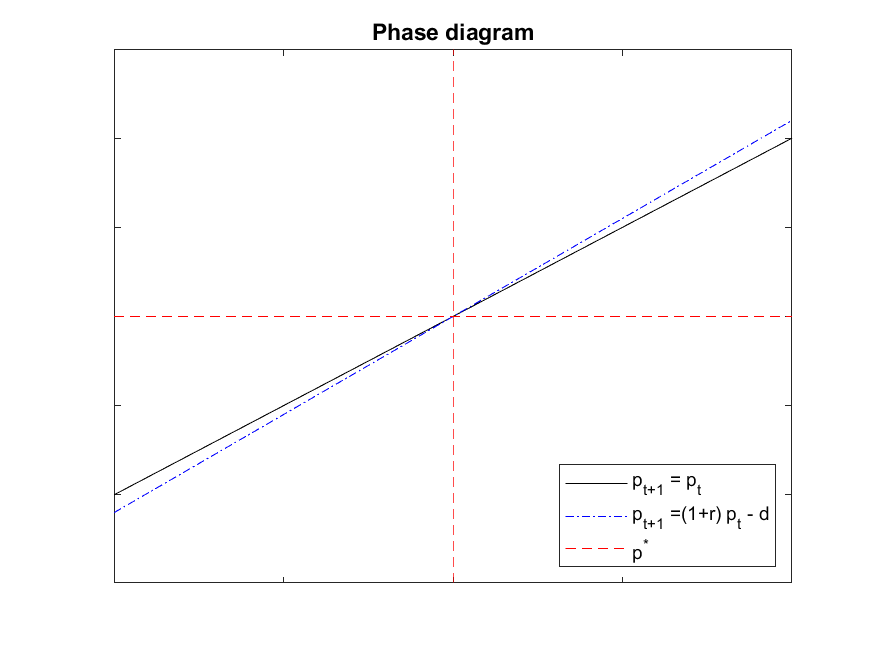
\includegraphics{phase} \\
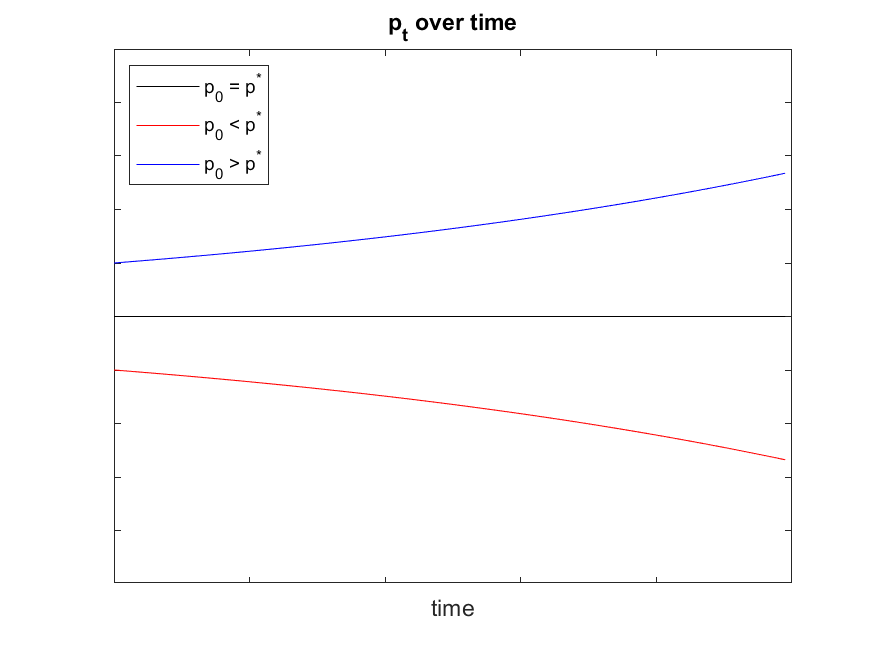
\includegraphics{pttime} \\

From the above phase diagram it is clear that any divergence from $p^{*}$ leads to continued movement away from the steady state. The same is shown in the chart of $p_t$ over time from initial values of $p$.

\section{Question 3}
Clearly, from the figures below, the stock price dynamics as calculated via Matlab act in precisely the same way as predicted in the previous question.

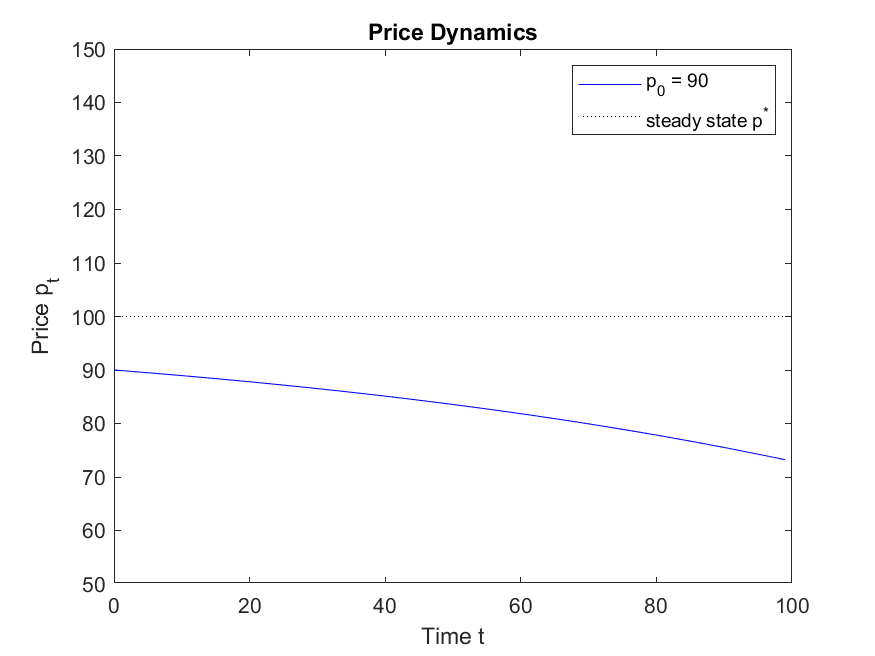
\includegraphics{dynamics_90} \\
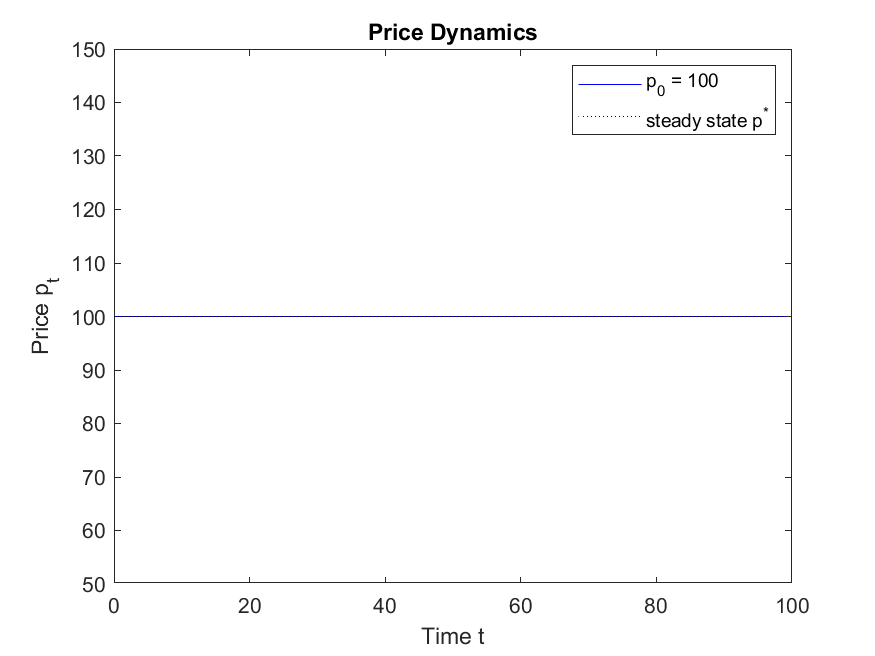
\includegraphics{dynamics_100} \\
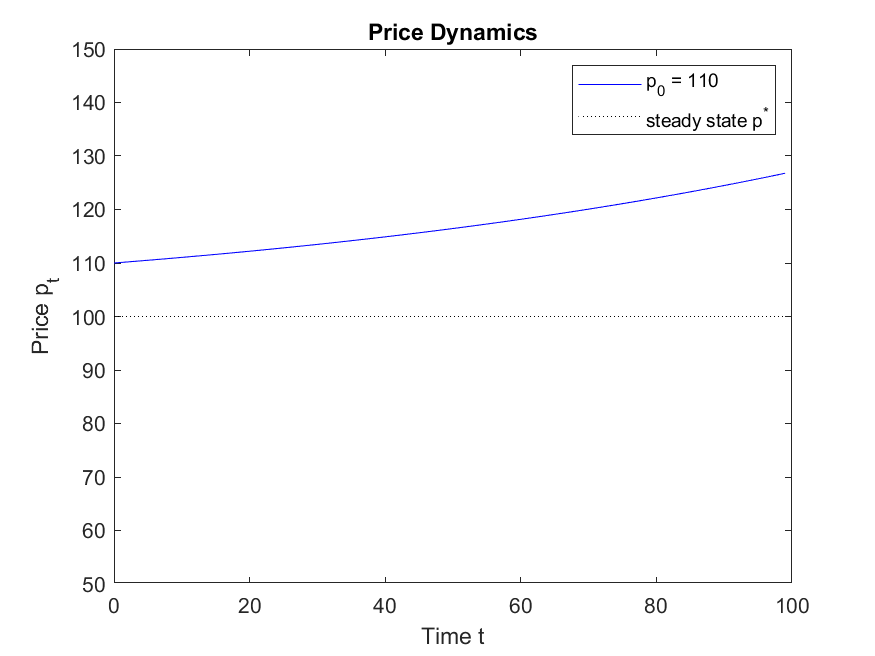
\includegraphics{dynamics_110} \\

\section{Question 4}
In this problem we are asked how the stock price would react to an FOMC announcement of a future interest rate hike. In this problem we are asked to rule out rational bubbles. In other words, our system will both begin and end at a steady state value. Note that these steady states will not be the same - at the beginning of the problem, $p^{*} = \frac{1}{0.01} = 100$ while at the end of the problem $p^{*} = \frac{1}{0.02} = 50.$ So, prior to the announcement, the stock price begins at its current steady state value of $100$. The announcement is made at $t=20$, and from that point until the interest rate changes at $t=50,$ the stock price transitions to the new steady state value of $50$, where it stays from $t=50$ and onwards.

It is clear then that the price dynamics of interest are the transition between the FOMC announcement and the interest rate hike. As the agents are perfectly rational and forward-looking, once the announcement is made they know what the price of the stock will be at $t=50$ and adjust the current stock price accordingly. Thus, we can solve backwards from $t=50$ through $t=20$ to find the price transition.

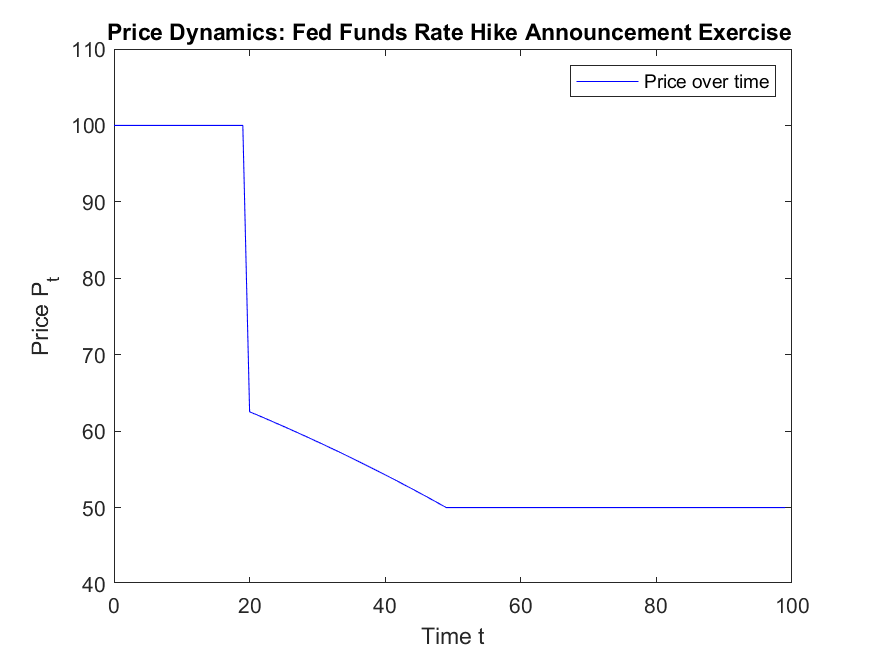
\includegraphics{dynamics_announcement} \\
From the above figure, it is clear that the stock price immediately plummets at the same period of the announcement - as the agents expect that the value of the stock at $t=50$ will be much lower than it had previously been priced as. After that point, the stock price slowly continues its movement towards its eventual valuation at $t=50$, where it remains for the rest of the exercise.
\end{document}
